% Options for packages loaded elsewhere
\PassOptionsToPackage{unicode}{hyperref}
\PassOptionsToPackage{hyphens}{url}
%
\documentclass[
  10pt,
  ignorenonframetext,
  aspectratio=169,t,xcolor=table]{beamer}
\usepackage{pgfpages}
\setbeamertemplate{caption}[numbered]
\setbeamertemplate{caption label separator}{: }
\setbeamercolor{caption name}{fg=normal text.fg}
\beamertemplatenavigationsymbolsempty
% Prevent slide breaks in the middle of a paragraph
\widowpenalties 1 10000
\raggedbottom
\setbeamertemplate{part page}{
  \centering
  \begin{beamercolorbox}[sep=16pt,center]{part title}
    \usebeamerfont{part title}\insertpart\par
  \end{beamercolorbox}
}
\setbeamertemplate{section page}{
  \centering
  \begin{beamercolorbox}[sep=12pt,center]{part title}
    \usebeamerfont{section title}\insertsection\par
  \end{beamercolorbox}
}
\setbeamertemplate{subsection page}{
  \centering
  \begin{beamercolorbox}[sep=8pt,center]{part title}
    \usebeamerfont{subsection title}\insertsubsection\par
  \end{beamercolorbox}
}
\AtBeginPart{
  \frame{\partpage}
}
\AtBeginSection{
  \ifbibliography
  \else
    \frame{\sectionpage}
  \fi
}
\AtBeginSubsection{
  \frame{\subsectionpage}
}
\usepackage{amsmath,amssymb}
\usepackage{iftex}
\ifPDFTeX
  \usepackage[T1]{fontenc}
  \usepackage[utf8]{inputenc}
  \usepackage{textcomp} % provide euro and other symbols
\else % if luatex or xetex
  \usepackage{unicode-math} % this also loads fontspec
  \defaultfontfeatures{Scale=MatchLowercase}
  \defaultfontfeatures[\rmfamily]{Ligatures=TeX,Scale=1}
\fi
\usepackage{lmodern}
\usecolortheme{beaver}
\ifPDFTeX\else
  % xetex/luatex font selection
\fi
% Use upquote if available, for straight quotes in verbatim environments
\IfFileExists{upquote.sty}{\usepackage{upquote}}{}
\IfFileExists{microtype.sty}{% use microtype if available
  \usepackage[]{microtype}
  \UseMicrotypeSet[protrusion]{basicmath} % disable protrusion for tt fonts
}{}
\makeatletter
\@ifundefined{KOMAClassName}{% if non-KOMA class
  \IfFileExists{parskip.sty}{%
    \usepackage{parskip}
  }{% else
    \setlength{\parindent}{0pt}
    \setlength{\parskip}{6pt plus 2pt minus 1pt}}
}{% if KOMA class
  \KOMAoptions{parskip=half}}
\makeatother
\usepackage{xcolor}
\newif\ifbibliography
\setlength{\emergencystretch}{3em} % prevent overfull lines
\providecommand{\tightlist}{%
  \setlength{\itemsep}{0pt}\setlength{\parskip}{0pt}}
\setcounter{secnumdepth}{-\maxdimen} % remove section numbering
%%%%%%%%%%%%%%%%%%%%%%%%%%%%%%%%%%%%%%%%%%%%%%%%%%%%%%%%%%%%%%%%%%%%%%%%%%%%%%%%%%%%%%%
%     <-- выше автоматическая преамбула  |  пользовательская преамбула ниже --->      %
%%%%%%%%%%%%%%%%%%%%%%%%%%%%%%%%%%%%%%%%%%%%%%%%%%%%%%%%%%%%%%%%%%%%%%%%%%%%%%%%%%%%%%%

%%% Работа с русским языком
\usepackage{cmap}					    % поиск в PDF
\usepackage{mathtext} 				% русские буквы в формулах

% Для разметки слайдов и картинок
\usepackage{tikz}
\usepackage{animate}

% Для двойных прямых кавычек в Verbatim (не работает почему-то)
\usepackage{upquote}

% % Работа с прочими шрифтами
% \usepackage{fontspec}      %% УЖЕ ЗАГРУЖЕН В ПРЕАМБУЛЕ подготавливает загрузку шрифтов Open Type, True Type и др.
\setmainfont{Times New Roman} %% задаёт основной шрифт документа
\setsansfont{Microsoft Sans Serif} %% задаёт шрифт без засечек
\setmonofont[Scale=0.7]{DejaVu Sans Mono} %% моноширинный шрифт\

%% математический шрифт
\setmathfont[version=Cambria]    {Cambria Math}
\setmathfont[version=LatinModern]{Latin Modern Math}
\mathversion{Cambria}

% Межстрочный интервал в verabtim
\makeatletter
\def\verbatim@font{\linespread{0.7}\normalfont\ttfamily}
\makeatother

% Межабзацный интервал в columns
\makeatletter
\newcommand{\@minipagerestore}{\setlength{\parskip}{4pt plus 2pt minus 1pt}}
\makeatother

% \usepackage{hyperref} %% УЖЕ ЗАГРУЖЕН В ПРЕАМБУЛЕ
\definecolor{links}{HTML}{2A1B81}
\hypersetup{colorlinks=true,linkcolor=,urlcolor=links,pdfview=FitH,pdfpagelayout=SinglePage, unicode=true,breaklinks=true}

% Тильда в тексте
\newcommand{\mytilde}{\char`~\:}
% argmin и argmax
\DeclareMathOperator*{\argmax}{argmax}
\DeclareMathOperator*{\argmin}{argmin}

% Более простой ввод команд для двухколоночной верстки
\newcommand{\columnsbegin}{\vspace{-0.5\baselineskip}\begin{columns}[t,onlytextwidth]}
\newcommand{\columnsend}{\end{columns}}
\newcommand{\columnbegin}{\begin{column}}
\newcommand{\columnend}{\end{column}}
\newcommand{\blockbegin}{\begin{block}}
\newcommand{\blockend}{\end{block}}

% allows to add alignment keys to \includegraphics
\usepackage[export]{adjustbox}

% Работа с таблицами %%%%%%%%%%%%%%

\usepackage{adjustbox}

% Новые типы колонок для окружения tabular, чтобы можно было задавать их ширину
% Например, \begin{tabular}{ L{2.3cm} C{2cm} C{1.5cm} C{2.5cm} C{4cm}}
\usepackage{array}
\renewcommand{\arraystretch}{1.5}
\newcolumntype{L}[1]{>{\raggedright\let\newline\\\arraybackslash\hspace{0pt}}m{#1}}
\newcolumntype{C}[1]{>{\centering\let\newline\\\arraybackslash\hspace{0pt}}m{#1}}
\newcolumntype{R}[1]{>{\raggedleft\let\newline\\\arraybackslash\hspace{0pt}}m{#1}}

% Для таблиц в tabularx окружении при помощи пакета huxtable
\usepackage{tabularx}

% Прочие настройки beamer %%%%%%%%%%%%

% Цвета
% Посмотреть и конвертировать можно здесь https://convertingcolors.com/
%                       RGB                       HEX    nearest R colour
\definecolor{spbblack}{RGB}{30,30,30}           % 1e1e1e "gray12"
\definecolor{spbgrey}{RGB}{191,191,191}         % BFBFBF "gray75"
\definecolor{spbteal}{RGB}{188, 216, 221}       % BCD8DD "powderblue"
\definecolor{spblightteal}{RGB}{222,236,238}    % DEECEE "azure2"
\definecolor{spbred}{RGB}{203,55,87}            % CB3757 "maroon"
\definecolor{spbgreen}{RGB}{168,207,166}        % A8CFA6 "darkseagreen3"
\definecolor{spbdarkgreen}{RGB}{96,157,131}     % 609D83 "paleturquoise4"
\definecolor{spbblue}{RGB}{98,122,235}          % 627AEB "cornflowerblue"
\definecolor{spbdarkblue}{RGB}{24,112,184}      % 1870B8 "dodgerblue3"
\definecolor{spbviolet}{RGB}{212,207,232}       % D4CFE8
\definecolor{spbdarkviolet}{RGB}{101,118,185}   % 6576B9
\definecolor{spbyellow}{RGB}{254,192,15}        % FEC00F "darkgoldenrod1"
\definecolor{spbsteelblue}{RGB}{70,130,180}     % 4682B4 "steelblue"


% Галочка в тексте
\def\checkmark{\tikz\fill[scale=0.4](0,.35) -- (.25,0) -- (1,.7) -- (.25,.15) -- cycle;}

% Для раскраски таблиц
\usepackage{colortbl}
% переопределяем tabular с раскраской
\let\oldtabular\tabular
\let\endoldtabular\endtabular
\renewenvironment{tabular}{
\setlength\arrayrulewidth{1pt} \arrayrulecolor{white}
\rowcolors{1}{spbteal}{spblightteal}
\oldtabular}{\endoldtabular}

\usepackage{caption}
\captionsetup[table]{name=Таблица}
% переопределяем tabularx с раскраской
\let\oldtabularx\tabularx
\let\endoldtabularx\endtabularx
\renewenvironment{tabularx}{
\setlength\arrayrulewidth{1pt} \arrayrulecolor{white}
\rowcolors{1}{spbteal}{spblightteal}
\oldtabularx}{\endoldtabularx}


% Для подсветки элементов формул
\usepackage[beamer,customcolors,norndcorners]{hf-tikz}
\hfsetfillcolor{spbteal}
\hfsetbordercolor{white}

\setbeamercolor{myfootlinetext}{fg=spbgrey}
\setbeamerfont{myfootlinetext}{size=\normalsize}
% Переопределяем бимеровский footline
\setbeamertemplate{footline}{
  % \vspace{1cm}
  \usebeamercolor[fg]{myfootlinetext}
  \usebeamerfont{myfootlinetext}
  \hspace{0.5cm}\textbf{\insertpagenumber}\hfill\strut\quad
  \vspace{0.4cm}
}

% Фон слайдов
\usepackage{etoolbox}
\makeatletter
\setbeamertemplate{background canvas}{%
   \ifnumequal{\c@framenumber}{1}{%
      % First frame
      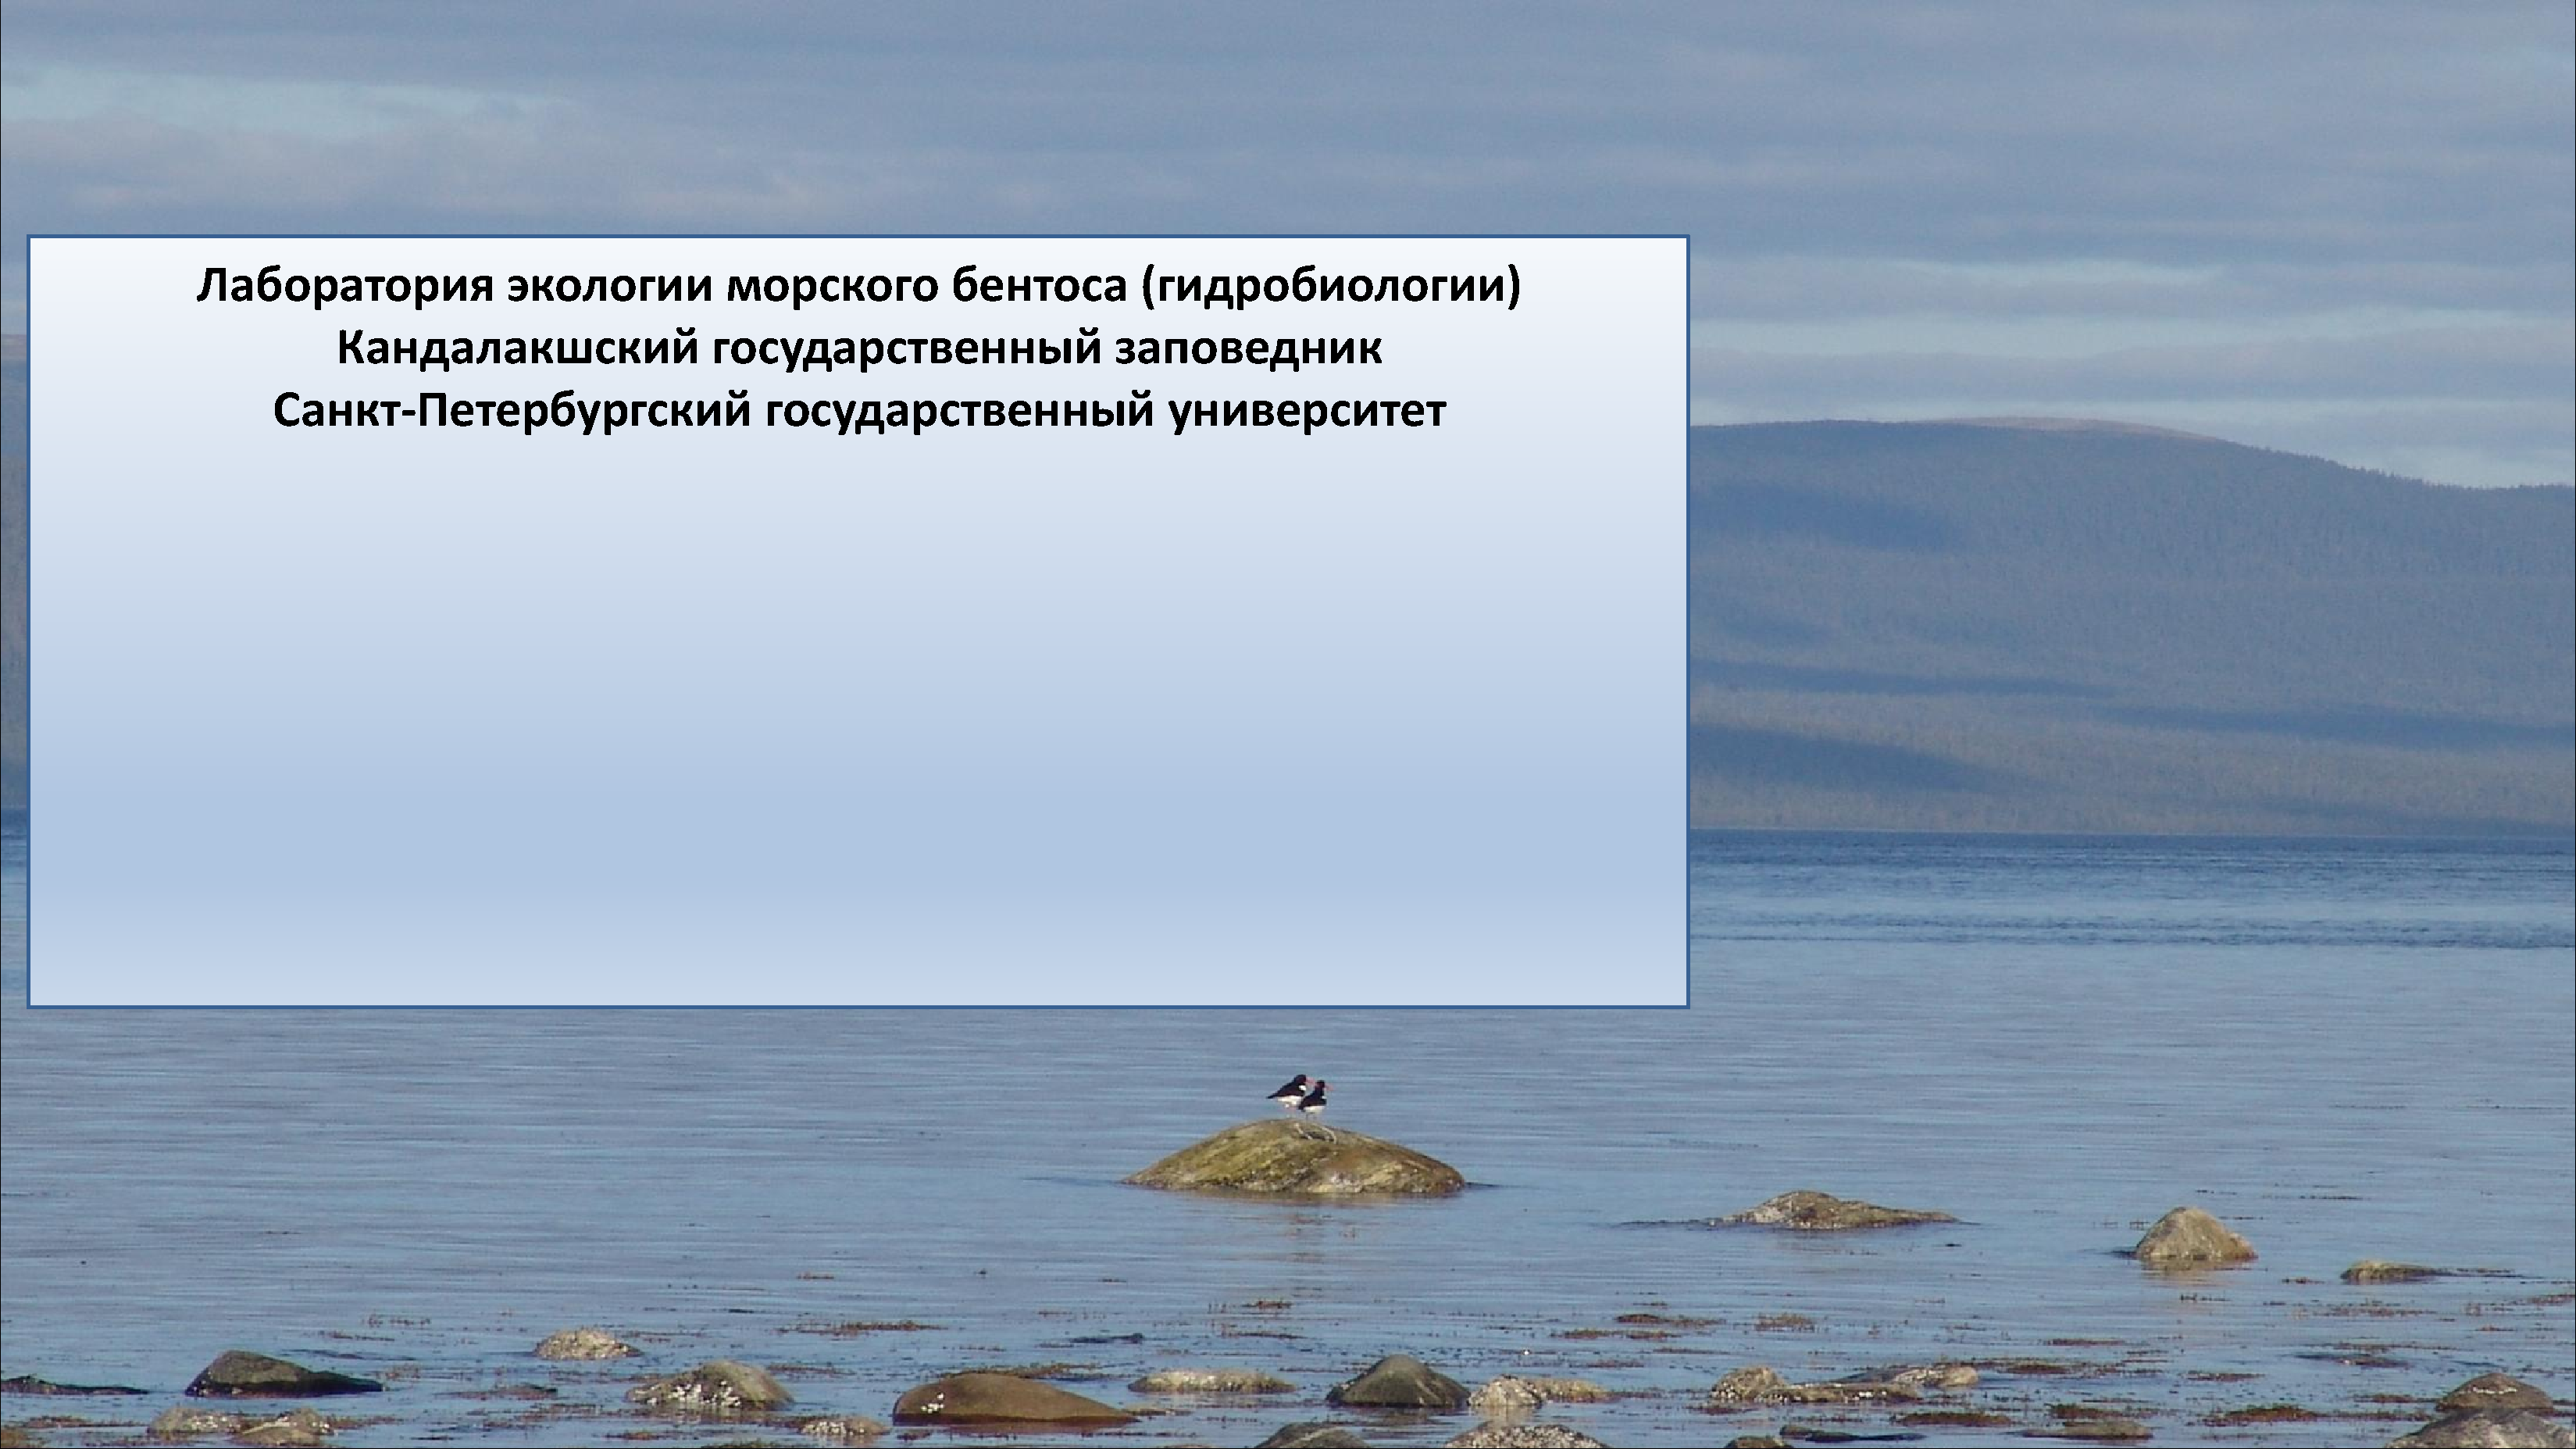
\includegraphics[width=\paperwidth,height=\paperheight]{includes/Primer_title.pdf}
   }{%
      \ifnumequal{\c@framenumber}{\inserttotalframenumber-1}{
         % Before last frame
         
\includegraphics[width=\paperwidth,height=\paperheight]{includes/Primer_sources.pdf}
      }{%
      \ifnumequal{\c@framenumber}{\inserttotalframenumber}{
         % Last frame
         
\includegraphics[width=\paperwidth,height=\paperheight]{includes/Primer_last.pdf}
      }{%
         % Other frames
         
\includegraphics[width=\paperwidth,height=\paperheight]{includes/Primer_slide.pdf}
      }%
   }%
   }%
}
\makeatother

% Разметка титульного слайда
\setbeamertemplate{title page}{%
    \begin{tikzpicture}[remember picture,overlay]
    % Заголовок
    \node[anchor=west]
    at ([yshift=-25mm,xshift=18mm]current page.north west) (title)
    {\parbox[b][1in]{0.45\paperwidth}{\raggedright%
            \usebeamerfont{title}\textcolor{spbblack}{\textbf\inserttitle}}};
    % Автор
    \node[anchor=west]
    at ([yshift=-57mm,xshift=18mm]current page.north west) (author)
    {\parbox[t][1in]{.45\paperwidth}{\raggedright%
            \usebeamerfont{author}\textcolor{spbblack}{\insertauthor}}};
    % Организация
    \node[anchor=north west]
    at ([yshift=37mm,xshift=18mm]current page.south west) (institute)
    {\parbox[t]{.45\paperwidth}{\raggedright%
            \usebeamerfont{institute}\textcolor{spbblack}{\insertinstitute}}};
    \end{tikzpicture}
}
% Заголовок на титульном слайде
\setbeamercolor{titlelike}{parent=palette primary,fg=spbblack,bg=}

% Блоки
\setbeamercolor{block title}{fg=spbblack, bg=}

% Заголовки слайдов
\setbeamercolor{frametitle}{bg=}
\setbeamertemplate{frametitle}{
  \vspace{1cm}
  \color{spbblack}\bfseries\insertframetitle%
}

% Маркеты элементов списка
\setbeamertemplate{itemize items}{\color{spbteal}\normalsize$\bullet$}


%%%%%%%%%%%%%%%%%%%%%%%%%%%%%%%%%%%%%%%%%%%%%%%%%%%%%%%%%%%%%%%%%%%%%%%%%%%%


%     <-- выше пользовательская преамбула | новый Verabtim ниже --->      %
%%%%%%%%%%%%%%%%%%%%%%%%%%%%%%%%%%%%%%%%%%%%%%%%%%%%%%%%%%%%%%%%%%%%%%%%%%%%%%%%%%%%%%%

% Уменьшаем интервалы сверху и снизу Verbatim
% https://stackoverflow.com/a/2319042
\setlength\partopsep{-\topsep}
\addtolength\partopsep{-\parskip}
\addtolength\partopsep{0.9\baselineskip}

% Линия рядом с кодом
\RecustomVerbatimEnvironment{Highlighting}{Verbatim}{
    commandchars=\\\{\},
    frame=leftline,
    framerule=0.75mm,
    rulecolor=\color{spbteal},
    samepage=true,
    baselinestretch=0.8
}

\usepackage{caption}

%%%%%%%%%%%%%%%%%%%%%%%%%%%%%%%%%%%%%%%%%%%%%%%%%%%%%%%%%%%%%%%%%%%%%%%%%%%%

\ifLuaTeX
  \usepackage{selnolig}  % disable illegal ligatures
\fi
\IfFileExists{bookmark.sty}{\usepackage{bookmark}}{\usepackage{hyperref}}
\IfFileExists{xurl.sty}{\usepackage{xurl}}{} % add URL line breaks if available
\urlstyle{same}
\hypersetup{
  hidelinks,
  pdfcreator={LaTeX via pandoc}}

\title{Основы литературного программирования}
\author{В.М. Хайтов, к.б.н.}
\date{}

\begin{document}
\frame{\titlepage}

\begin{frame}{Литературное программирование}
\protect\hypertarget{ux43bux438ux442ux435ux440ux430ux442ux443ux440ux43dux43eux435-ux43fux440ux43eux433ux440ux430ux43cux43cux438ux440ux43eux432ux430ux43dux438ux435}{}
В.М. Хайтов, к.б.н.

\insertinstitute
\end{frame}

\begin{frame}{Для исполнителей}
\protect\hypertarget{ux434ux43bux44f-ux438ux441ux43fux43eux43bux43dux438ux442ux435ux43bux435ux439}{}
\columnsbegin
\column{0.48\textwidth}


\includegraphics[height=0.6\textheight,keepaspectratio]{./images/stock-photo-angry-boss-standing-opposite-his-secretary-631514021.jpg}

\column{0.48 \textwidth}

Вы создали презентацию, написали текст статьи или отчета.

Начальнику не понравилась форма графиков, цвет заливки, величина шрифта
и т. п\ldots{}

В дополнение коллеги принели вам исправленные файлы с первичными
данными\ldots{}

Все документы надо срочно переделывать\ldots{}

\columnsend

\centering

Выход из этого кошмара --- создание RMD-документа.
\end{frame}

\begin{frame}{Для пользователей разных платформ}
\protect\hypertarget{ux434ux43bux44f-ux43fux43eux43bux44cux437ux43eux432ux430ux442ux435ux43bux435ux439-ux440ux430ux437ux43dux44bux445-ux43fux43bux430ux442ux444ux43eux440ux43c}{}
\columnsbegin
\column{0.48\textwidth}


\includegraphics[height=0.6\textheight,keepaspectratio]{./images/stock-photo-moscow-russia-december-road-signs-with-top-brand-operating-system-logos-android-mac-770756293.jpg}

\column{0.48 \textwidth}

Ваши коллеги работают под Linux и Windows, а вы предпочитаете Mac OS.

Продукт вашего совместного творчества должен читаться на любом
компьютере.

\columnsend

\centering

Основа плодотворного сотрудничества --- работа с RMD-документами.
\end{frame}

\begin{frame}{Для исследователей}
\protect\hypertarget{ux434ux43bux44f-ux438ux441ux441ux43bux435ux434ux43eux432ux430ux442ux435ux43bux435ux439}{}
\columnsbegin
\column{0.48\textwidth}


\includegraphics[height=0.6\textheight,keepaspectratio]{./images/stock-photo-businessman-interacting-with-a-hud-interface-against-a-blurred-blue-background-graphs-toned-image-1017564916.jpg}

\column{0.48 \textwidth}

Вы ученый-иследователь.

В статьях, которые вы читаете, видна лишь вершина айсберга: характер
данных, процедуры анализа, способ построения таблиц и графиков остаются
в тени.

Вас не оставляет чувство сомнения в правоте автора статьи, так как нет
возможности воспроизвести те действия с данными, которые произвел автор.

\columnsend

\centering

Выход из этого --- стать сторонником идеи \textbf{Reproducible research}
\end{frame}

\begin{frame}{Reproducible research}
\protect\hypertarget{reproducible-research}{}
Воспроизводимое исследование --- это анализ, который может быть
воспроизведен на основе тех же данных любым другим исследователем.

Воспроизводимое исследование не надо путать с воспроизводимостью
результатов!
\end{frame}

\begin{frame}{Reproducible research}
\protect\hypertarget{reproducible-research-1}{}
\textbf{Критерии воспроизводимого исследования}

\begin{enumerate}
  \item Исходные данные (raw data) доступны любому читателю-потребителю (в идеале, публично доступны).
  \item Все методы анализа полностью описаны.
  \item Весь процесс анализа исходных данных (от чтения данных до финального результата) полностью описан и сохранен в виде некоторого текста (кода анализа).

\end{enumerate}

\centering

Лучшее средство для представления своих результатов как воспроизводимого
исследования --- это создание RMD-документов.
\end{frame}

\begin{frame}{Создание RMD-документа}
\protect\hypertarget{ux441ux43eux437ux434ux430ux43dux438ux435-rmd-ux434ux43eux43aux443ux43cux435ux43dux442ux430}{}
В.М. Хайтов, к.б.н.

\insertinstitute
\end{frame}

\begin{frame}{R Markdown}
\protect\hypertarget{r-markdown}{}
\columnsbegin
\column{0.6\textwidth}

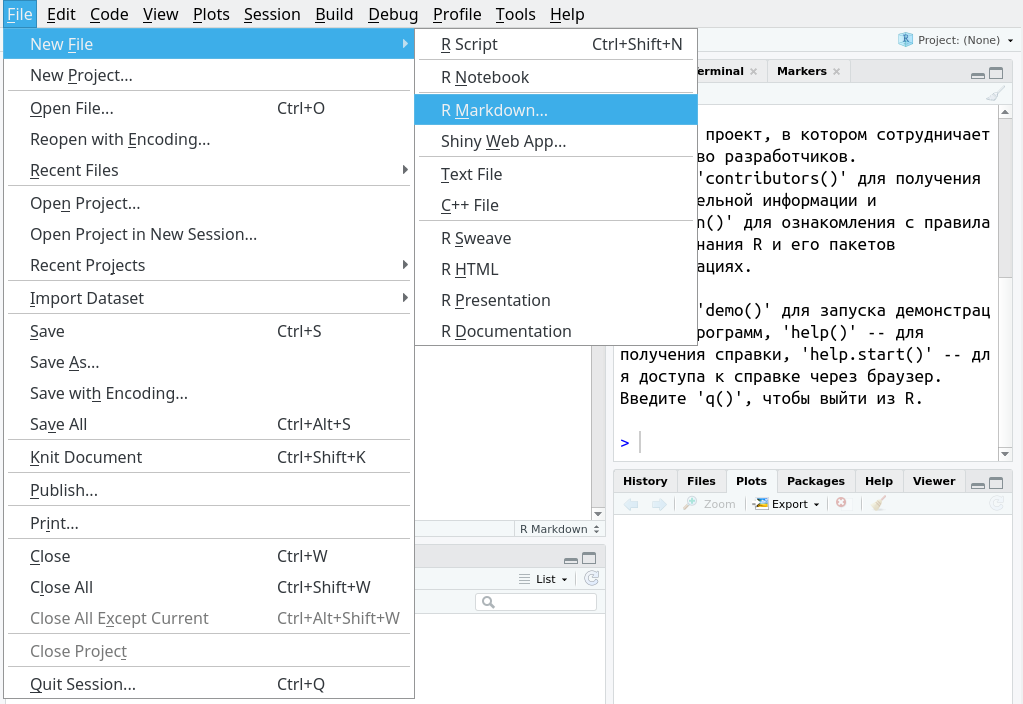
\includegraphics[height=0.7\textheight,keepaspectratio]{./images/RMD_step_1_Ira.png}

\column{0.4\textwidth}

RMD-документы --- это документы, созданные с использованием языка
разметки R Markdown.

\columnsend
\end{frame}

\begin{frame}{Документ или презентация}
\protect\hypertarget{ux434ux43eux43aux443ux43cux435ux43dux442-ux438ux43bux438-ux43fux440ux435ux437ux435ux43dux442ux430ux446ux438ux44f}{}
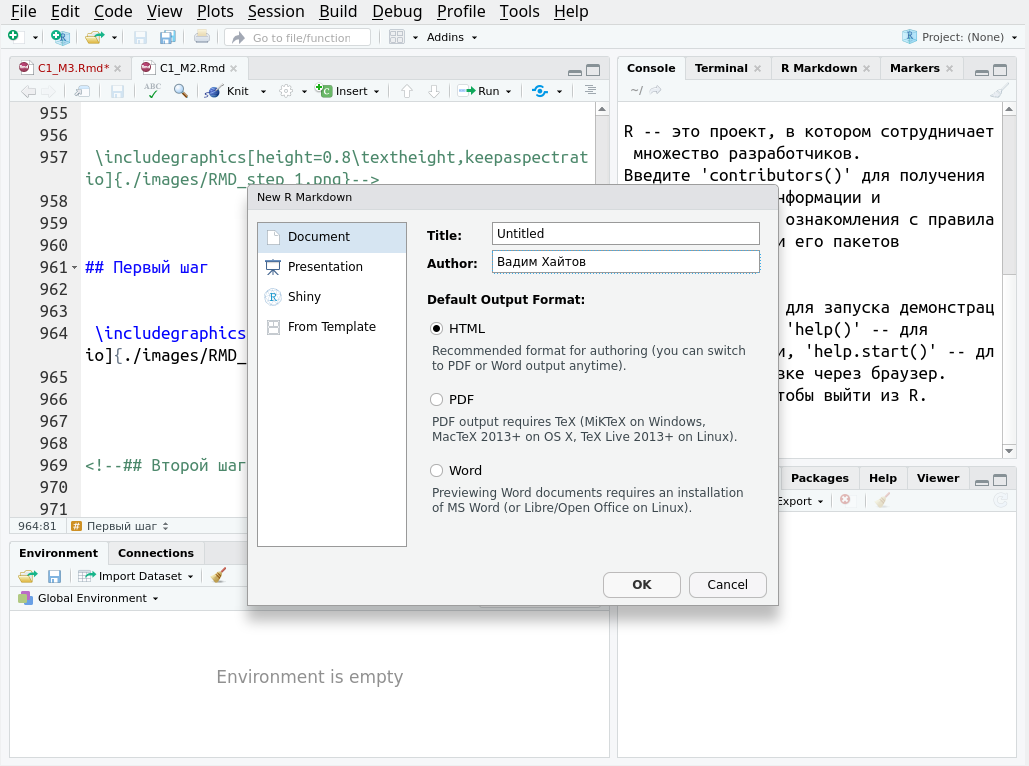
\includegraphics[height=0.7\textheight,keepaspectratio]{./images/RMD_step_2_Ira.png}
\end{frame}

\begin{frame}{Внешний вид RMD-документа}
\protect\hypertarget{ux432ux43dux435ux448ux43dux438ux439-ux432ux438ux434-rmd-ux434ux43eux43aux443ux43cux435ux43dux442ux430}{}
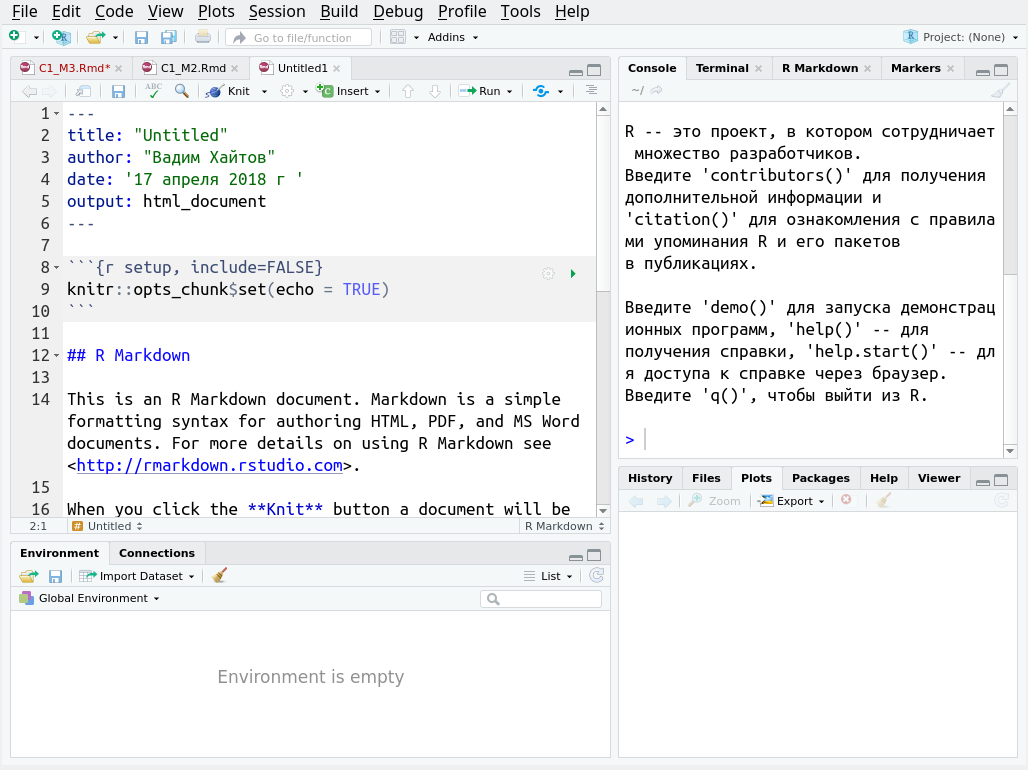
\includegraphics[height=0.7\textheight,keepaspectratio]{./images/RMD_step_3_Ira.png}
\end{frame}

\begin{frame}[fragile]{Создание итогового документа}
\protect\hypertarget{ux441ux43eux437ux434ux430ux43dux438ux435-ux438ux442ux43eux433ux43eux432ux43eux433ux43e-ux434ux43eux43aux443ux43cux435ux43dux442ux430}{}
Текст RMD-документа передается функции \texttt{knit()} из пакета
\texttt{knitr}.

Эта функция создает итоговый документ в том формате, который указан в
заголовке RMD-документа (html, pdf, docx).
\end{frame}

\begin{frame}{Чанки}
\protect\hypertarget{ux447ux430ux43dux43aux438}{}
\columnsbegin
\column{0.6\textwidth}

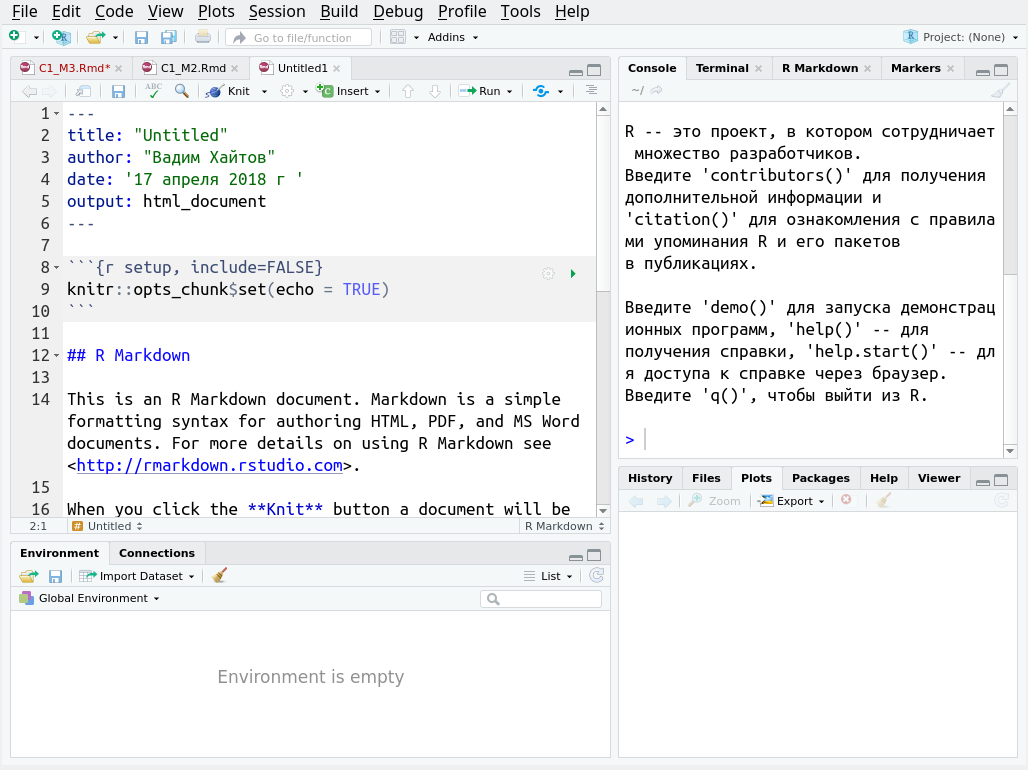
\includegraphics[height=0.7\textheight,keepaspectratio]{./images/RMD_step_3_Ira.png}

\column{0.4\textwidth}

Чанк --- это исполняемый код, встроенный в текст.

Вставка чанка в RStudio: Ctrl+Alt+I

\columnsend
\end{frame}

\begin{frame}{Пример RMD-документа}
\protect\hypertarget{ux43fux440ux438ux43cux435ux440-rmd-ux434ux43eux43aux443ux43cux435ux43dux442ux430}{}
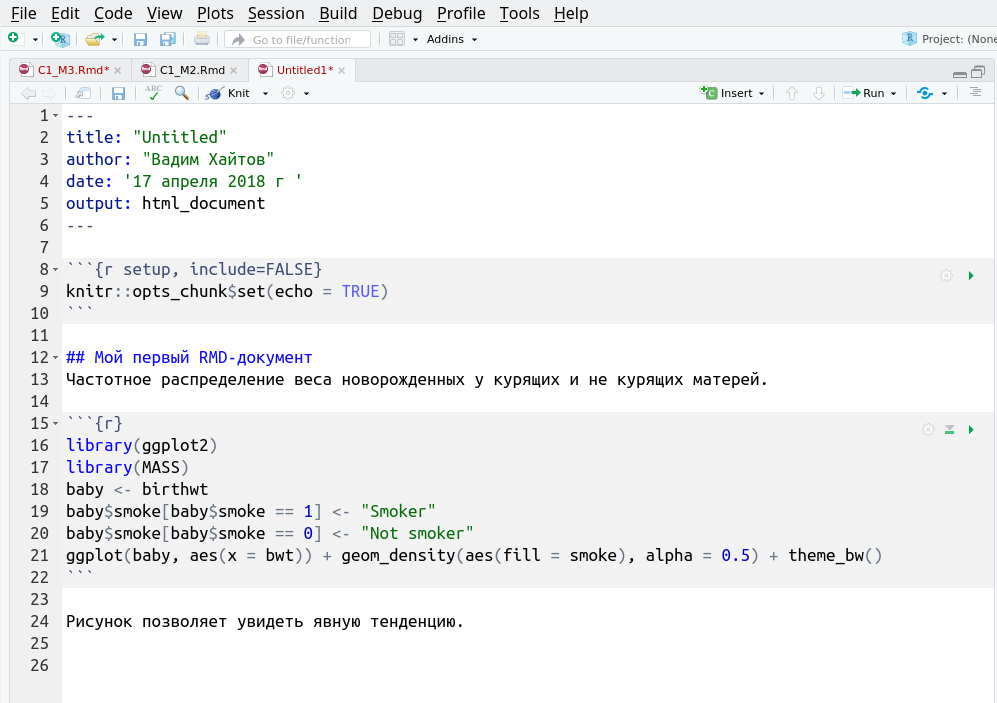
\includegraphics[height=0.7\textheight,keepaspectratio]{./images/RMD_example_Ira.png}
\end{frame}

\begin{frame}[fragile]{Результат работы \texttt{knitr} в окне браузера}
\protect\hypertarget{ux440ux435ux437ux443ux43bux44cux442ux430ux442-ux440ux430ux431ux43eux442ux44b-knitr-ux432-ux43eux43aux43dux435-ux431ux440ux430ux443ux437ux435ux440ux430}{}
\columnsbegin
\column{0.6\textwidth}

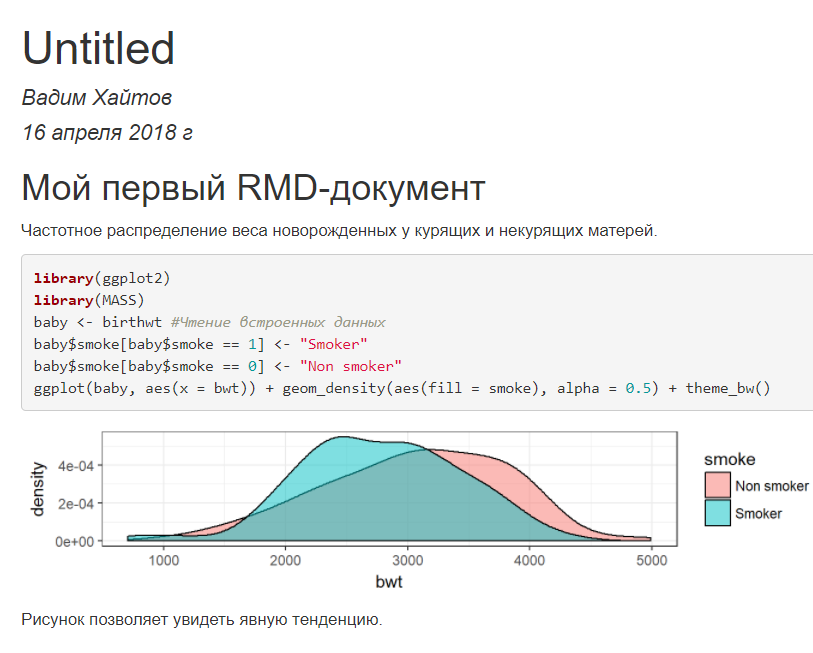
\includegraphics[height=0.7\textheight,keepaspectratio]{./images/RMD_browser_view.png}

\column{0.4\textwidth}

В результате работы \texttt{knitr} появляется html-файл, который можно
просмотреть в обычном браузере.

\columnsend
\end{frame}

\begin{frame}{Параметры чанков}
\protect\hypertarget{ux43fux430ux440ux430ux43cux435ux442ux440ux44b-ux447ux430ux43dux43aux43eux432}{}
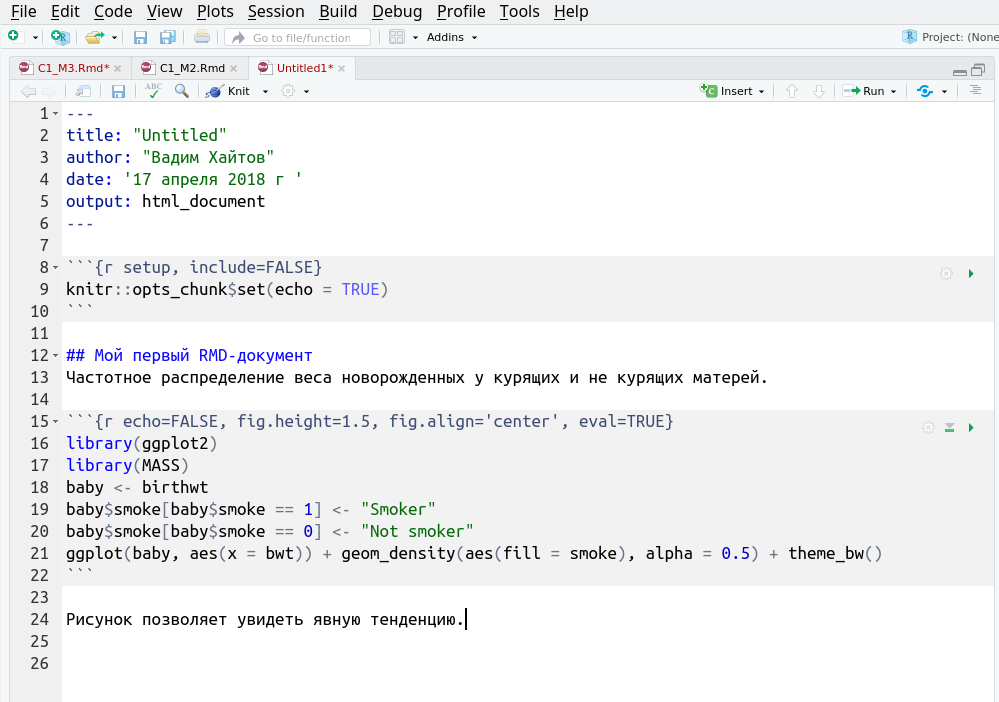
\includegraphics[height=0.7\textheight,keepaspectratio]{./images/RMD_chunk_parameters_Ira.png}
\end{frame}

\begin{frame}{Результат работы \texttt{knitr} с новыми параметрами
чанка}
\protect\hypertarget{ux440ux435ux437ux443ux43bux44cux442ux430ux442-ux440ux430ux431ux43eux442ux44b-knitr-ux441-ux43dux43eux432ux44bux43cux438-ux43fux430ux440ux430ux43cux435ux442ux440ux430ux43cux438-ux447ux430ux43dux43aux430}{}
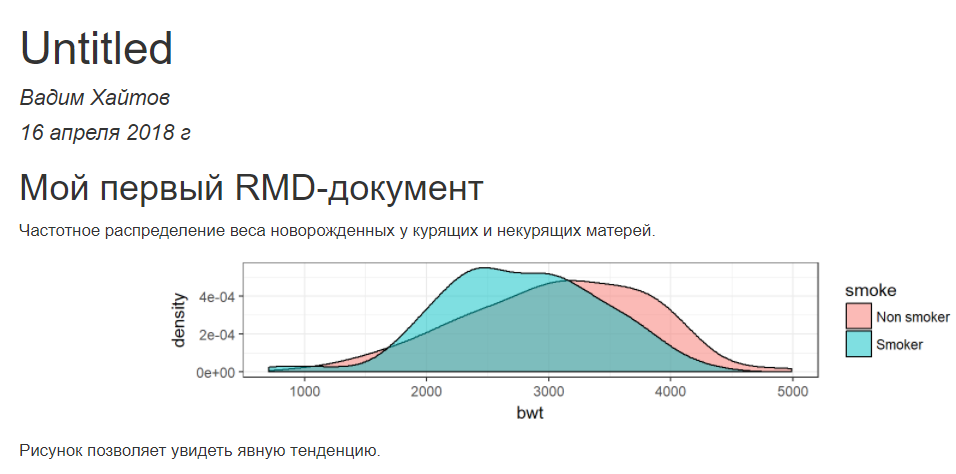
\includegraphics[height=0.7\textheight,keepaspectratio]{./images/RMD_browser_view_2.png}
\end{frame}

\begin{frame}[fragile]{Наиболее важные параметры чанка}
\protect\hypertarget{ux43dux430ux438ux431ux43eux43bux435ux435-ux432ux430ux436ux43dux44bux435-ux43fux430ux440ux430ux43cux435ux442ux440ux44b-ux447ux430ux43dux43aux430}{}
\begin{itemize}
\tightlist
\item
  \texttt{echo} --- Приводить ли код из чанка в документе, который
  получится в результате работы \texttt{knitr}
\item
  \texttt{eval} --- Запускать ли код, приведенный в чанке
\item
  \texttt{fig.} --- Набор параметров для регуляции положения и размера
  рисунков
\item
  \texttt{warning} --- Выводить ли в итоговый документ предупреждающие
  сообщения функций
\end{itemize}
\end{frame}

\begin{frame}
\end{frame}

\end{document}
